%!TEX program = xelatex
% 完整编译: xelatex -> bibtex -> xelatex -> xelatex
\documentclass[lang=cn,11pt,a4paper,cite=authoryear]{elegantpaper}

\title{软件工程课程设计报告}
\author{王宇航 \\ 南京农业大学 \and 毛亚琛 \\ 南京农业大学 \and 朱志畅 \\ 南京农业大学}

\date{\zhtoday}


% 本文档命令
\usepackage[section]{placeins}
\usepackage[final]{pdfpages}
\usepackage{array}
\graphicspath{{../../活动图/out/}{../../类图/out/}{../../设计类图/out/}{../../时序图/out/}{../../用例图/out/}}
\renewcommand{\listfigurename}{\mbox{}\hfill 插图 \hfill\mbox{}}
\renewcommand{\contentsname}{\mbox{}\hfill 目录 \hfill\mbox{}}
\hypersetup{hidelinks}

\begin{document}


\includepdf[]{cover.pdf}

\tableofcontents
\listoffigures

\maketitle

\section{需求分析及开发背景}

\subsection{绪论}

随着互联网与社会的发展,移动端技术日趋成熟,人们日趋注重自己的业余时间,在一个假期或者休闲时间旅游度假,也成为了这个时代的潮流。随着旅游业的迅速发展,各个城市之间的人口流动越来越频繁,在此条件之下,酒店住宿业也呈现出越来越火爆的趋势。而这其中,民宿房屋的租赁业务也变得越来越活跃。民宿房屋的预定系统,就是让人们可以在互联网上进行.民宿的预定和招租,为租客和房东都提供很多的便利。利用日趋成熟的移动端技术,带给人们生活中的便利,这正是时代所需。

\subsection{项目背景}

\subsubsection{民宿的概念}

什么是民宿?民宿是指利用自用住宅空闲房间,结合当地人文、自然景观、生态、环境资源及农林渔牧生产活动,为外出郊游或远行的旅客提供个性化住宿场所。除了一般常见的饭店以及旅社之外,其它可以提供旅客住宿的地方,例如民宅、休闲中心、农庄、农舍、牧场等,都可以归纳成民宿类。而民宿的产生是必然的,并不偶发于日本或中国台湾,世界各地都可看到类似性质的服务,民宿这个名字,在世界各国会因环境与文化生活不同而略有差异,欧洲方面多是采农庄式民宿(Accommodation in the Farm)经营,让一般民宿能够舒适地享受农庄式田园生活环境,体验农庄生活;加拿大则是采假日农庄(Vacation Farm)的模式,提供一般民宿假日可以享受农庄生活;美国都多见居家式民宿(Homestay)或青年旅舍(Hostel),不刻意布置的居家住宿,价格相对饭店便宜的住宿选择;英国则惯称Bed and Breakfast(BNB),按字面解释,意谓提供睡觉的地区以及简单早餐,索费大多每人每晚约二、三十英镑,视星级而定,当然价格会比一般旅馆便宜许多。

\subsubsection{国内外民宿的发展现状}

民宿出租在近几年愈发的变得火热,尤其在欧美市场,度假租赁异常火爆。中国游客在全世界范围内正逐渐赶超德国游客而变成全球最爱旅游的游客。随着经济情况越来越好,旅游黄金周各大景区的记录也在不断的被刷新着,其中自驾游和家庭游也逐渐成为了一种重要的旅游方式。在新浪乐居工作的罗军发现了中国有非常多的空闲房源可以利用,根据国务院的统计,有2.2亿套的中国房地产为沉淀房,其中有5000多套的空置房源,这说明了在中国民宿租赁会有特别大的市场。

民宿租赁主要在一些旅游城市发展的十分迅速,如北京,上海,杭州,深圳等等。途家租房是我国民宿租赁app的主力军,其中主要包括了两种房源,一种是其自营的房源,而另一种就是当地的民宿租赁。途家网是一家创立于2011年的新型公司,其主营业务为结合线下旅游,线中呼叫服务,线上度假公寓预定的在线订房交易平台系统。途家网由众多来自世界500强企业的精英组成,专注于创新科技和资源整合,为来自世界各地的旅行者提供了优质的服务和新的度假体验。同时,途家网也与携程网保持了战略合作关系,技术实力雄厚。

而在国外,最流行的民宿租赁当属airbnb。Airbnb是一家创立于美国的在线短租平台,是世界范围内民宿租赁的佼佼者,领头羊。该公司致力于将传统的民宿租赁业务结合互联网的创新技术发展到线上,从而减少房屋拥有者的管理难度。现如今,Airbnb的公司业务已经扩展到167个国家的近8000个地区,是真正的民宿租赁行业中的巨头。该公司的市值已达25亿美金,通过不断的融资,这个数字还会继续增长。

\subsubsection{民宿预定系统}

社会发展越来越快的今天,人们的生活水平也有了很大的提高。在我国,城市居民已经开始了高水准的休闲度假消费。伴随着旅游业的高速发展,新的住宿形式也在悄然兴起。民宿就是其中占比较大的类型,该类房间属于比较贴近生活的各种住宅小区,相较于酒店,它价格低廉,性价比极高。对于出差的小公司职员,旅游的学生,精打细算的顾客都是其庞大的客户群体。民宿在很大的程度上,既方便了租客,又方便了有闲置房屋的房东,可以说是两方互利。

通过在线的民宿房屋的预定系统,房东可以把空闲房屋的信息发布到服务器上,在app端进行显示,如可出租几天,地点,价格等等。而租客可以在app上对信息进行筛选,从而找到合适的房子进行短租。一般来说,民宿的出租与宾馆或者星级酒店相比设施更加完善齐全,而且价格更低,对于可以相互短租的用户来说,还可以直接进行互换,而不用收取短租的费用,经济且方便快捷。

互联网已经渗透到了人们生活中的方方面面,而智能手机的价格也是逐年走低,随着5G网络的飞速发展,用智能手机上网活动变得更加地方便。基于以上的一些客观条件,证明了民宿房屋的预定系统正是我们的时代所需,可以更好的方便人们的生活。

\subsection{需求分析}

\subsubsection{可行性分析}

可行性分析是构建系统之前重要的分析步骤,通过对系统各个方面的评估,包括经济、技术、前景等来研究系统构建成功的可能性。通过可行性分析,可以提早的发现设计过程中出现的错误和产生的漏洞,已避免可能出现的损失,规避风险。在开始开发整个程序之前进行整体的评估,发现问题时就降低了开发开始后的出现问题的风险,节约了不必要的时间花销,金钱花销,是开发系统的流程中必不可少的一个过程。

\subsubsection{经济可行性分析}

随着互联网技术和人们生活水平的提高,现阶段我国旅游市场呈现出越来越火爆的趋势,民宿房屋租赁市场有兴起的趋势。开发出一款好的民宿房屋租赁系统,可以帮助人们解决房屋租赁问题,提高房屋业主的房屋使用率,创造收益,同时也使得租客有更为方便快捷的租赁体验。

构建一个民宿房屋租赁系统仅需要培养较少的系统管理员,就可以维持系统的正常运行,使得用户和房屋业主都可以从中获得便利。综上所述,从经济的可行性角度来看,一款民宿房屋租赁系统是有着非常好的市场前景及非常高的经济价值,可以拉动民宿行业的发展,方便空闲房屋的利用与管理。

\subsubsection{技术可行性分析}

我们站在技术可行性的角度进行分析,现今市场上的Android等技术还是非常的成熟的。市场上的airbnb,途家等房屋租赁软件也是在良好的运行当中,因此就技术上来说,并不存在什么难点。现如今,随着Android技术的快速发展,我国的Android开发市场也呈现出越来越火爆的趋势,网上诸如极客学院,慕课网等在线教育的发展也为开发提供了非常大的便利,使得开发人员在学习方面非常的方便,所提出的问题也基本都能得到迅速的解答。因此,从技术可行性的角度来看,民宿房屋的预定系统是可行的。

\subsection{功能需求分析}

\subsubsection{业务逻辑分析}

本系统主要分为两大部分的设计,一部分为用户和房屋业主使用的客户端,另一部分为服务器端。

\begin{enumerate}
    \def\labelenumi{\arabic{enumi}.}
    \item
          用户通过客户端来进行系统的登陆,通过输入自己所需的房屋的信息来进行查找筛选等活动。
    \item
          用户通过客户端对所需的房屋进行下订单预订等活动,如果选择的信息为在线支付,则进入在线支付环节。如果选择的信息为到店付款,则直接进行确认订单。
    \item
          用户在完成房屋预定订单结束之后,房屋业主通过客户端直接收到用户的下单信息,完成房屋的预留确认环节。
\end{enumerate}

\subsubsection{系统功能分析}

在我们对本系统的进行了如上的业务逻辑分析之后,确认了本系统的功能基本分为两大部分:一部分是手机客户端的设计,另一部分则是后台服务器端管理界面的设计。手机客户端采用了时下流行的C/S架构设计,而后台服务器端则是采用了B/S架构进行设计,也就是说用户通过手机客户端访问系统,进行一系列所需的操作,而系统管理员则通过后台服务器端对系统进行维护管理。

对手机客户端来说,主要有如下的几大模块:用户登录注册模块,查询模块,订单管理模块,用户浏览模块,用户预约模块,支付定金模块以及发布租赁信息模块。

\begin{enumerate}
    \def\labelenumi{\arabic{enumi}.}
    \item
          \textbf{用户登录注册模块}

          用户在进行民宿租赁等操作之前需要先进行系统登录。对于未注册的用户来说需要进行注册,注册需要对手机号码进行神风验证,通过进行手机验证码来确认注册是否成功,同时也包括了密码找回等功能。
    \item
          \textbf{查询模块}

          用户可以进行民宿房屋信息查找等操作。民宿房屋的信息包括房屋的位置,出租的时间,出租的价格,房屋的内部配置等等。用户可以通过信息搜索,找寻筛选自己心仪的房屋,并进行收藏等操作。同时,查询功能也支持进行模糊查找。
    \item
          \textbf{订单管理模块}

          用户可以对已经形成的订单进行管理,查看订单进行的状态。可以对已经形成的订单进行查看、删除、支付等操作。
    \item
          \textbf{用户浏览模块}

          用户可以对客户端里的房屋信息进行浏览,包括房屋的图片、位置、设施等情况。同时,用户还可以查看其它用户对该房屋的评价,在登录状态下,用户也可以对自己租赁过的房屋进行评价。
    \item
          \textbf{用户预约模块}

          用户可以通过预约按钮来对已经选中的民宿房屋进行预约。预约时要确保用户的登陆状态,输入用户的入住时间,入住时长,入住人个人信息,手机号码等信息。确认预约成功后,将会给租赁用户和房屋拥有者发送信息,以确认订单的正确性。
    \item
          \textbf{支付定金模块}

          用户在进行预约民宿房屋的操作之后,可以通过手机来支付定金,该模块同时支持现今主流的支付方式,如支付宝支付等。支付定金后房屋将会锁定,为租客进行保留。
    \item
          \textbf{发布租赁信息模块}

          对于房屋业主来说,还需要有发布租赁信息的功能,包括了填写房屋地点,租赁的时间、价格,房屋的配套设施等信息。
\end{enumerate}

对于后台服务器端来说,主要有如下几大模块:个人信息管理模块,房屋信息管理。模块,预约管理模块,租房记录管理模块,租客信息管理模块。

\begin{enumerate}
    \def\labelenumi{\arabic{enumi}.}
    \item
          \textbf{个人信息管理模块}

          该模块包括了普通用户与房屋业主的个人信息,可以在此进行对于违规用户的封禁操作。
    \item
          \textbf{房屋信息管理模块}

          该模块包括了正在出租和处在租赁状态中的房屋信息,管理员可以在此对这些状态进行管理。
    \item
          \textbf{预约管理模块}

          该模块包括了普通用户和房屋之间的预约信息,管理员可以查看,也可以通过增加或者删除来手动的对其进行管理。
    \item
          \textbf{租房记录管理模块}

          该模块包含了用户的房租租赁信息记录,管理员可以查看,也可以通过删除操作来手动的对其进行管理。
    \item
          \textbf{租客信息管理模块}

          该模块包含了房屋的历史租客的信息,管理员可以查看,也可以通过删除操作来手动的对其进行管理。
\end{enumerate}

\subsection{性能需求分析}

对于一个app应用来说,高峰时系统能够承载的并发请求是衡量这个系统性能的关键标志,能同时处理大量的峰值请求,是该系统需要考虑的。通过一个叫每秒请求数(Requests
per
second)的概念,我们来衡量系统的负载能力。通常的对于一个系统来说,增加并发用户数量的时候每秒请求数量也会增加。然而,我们终究会达到一个并发用户数量开始压倒服务器的临界点,如果继续增加并发用户的数量,每秒请求数量则会开始下降,而相应的反应时间将会增加。

一般的来说,带宽和硬件配置是决定系统负载能力的决定性因素。我们需要将关注.的重点放在一定带宽和硬件配置的基础设施之上,从而使系统的负载能力达到最大化。系统部署所在的服务器的硬件决定了一个系统的最大负载能力,也是系统的上限。cpu频率/核数,内存大小以及速度,硬盘速度都起着至关重要的作用。

\section{用例图}

用例图是指由参与者、用例,边界以及它们之间的关系构成的用于描述系统功能的视图。用例图是外部用户(被称为参与者)所能观察到的系统功能的模型图。用例图是系统的蓝图。用例图呈现了一些参与者,一些用例,以及它们之间的关系,主要用于对系统、子系统或类的功能行为进行建模。
系统的用例图包含账号管理、订单管理。账号管理包括账号的注册(其中包括手机号注册和邮箱注册),订单管理包含着对订单的操作。
房东部分用例图包含民宿管理和上架民宿。民宿管理部分包括修改价格、更新房源和下架。上架民宿包含着房源信息提交以及房东信息审核。
房客部分包含着检索民宿和预订民宿,其中检索民宿包含着模糊检索和精确检索,预定民宿可以拓展为优惠预订。

\begin{figure}[]
    \centering
    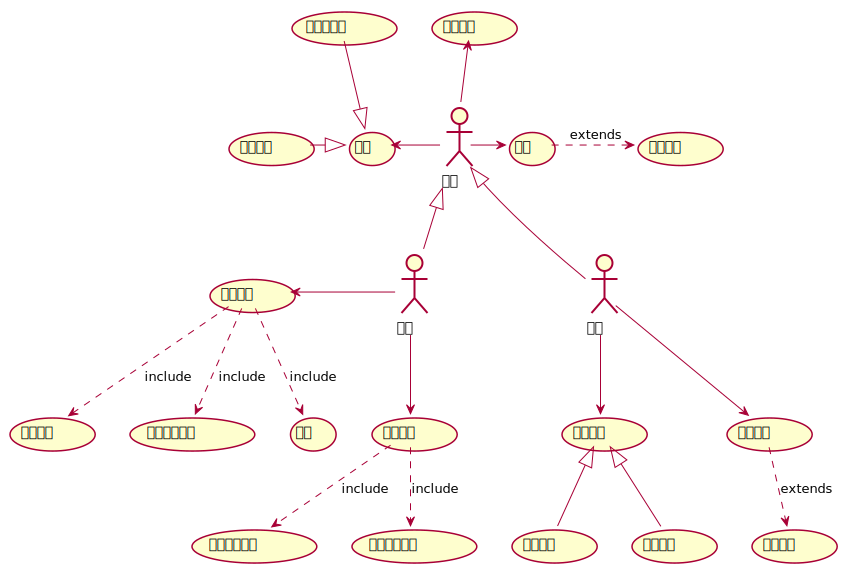
\includegraphics[width=0.8\textwidth]{用例图.pdf}
    \caption{用例图}
    \label{fig:用例图}
\end{figure}

\section{类图}

类图是显示了模型的静态结构,特别是模型中存在的类、类的内部结构以及它们与其他类的关系等。类图不显示暂时性的信息。类图是面向对象建模的主要组成部分。它既用于应用程序的系统分类的一般概念建模,也用于详细建模,将模型转换成编程代码。类图也可用于数据建模。总体类图如\figref{fig:类图}。

\begin{figure}[]
    \centering
    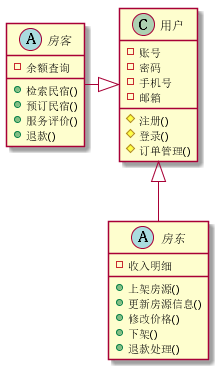
\includegraphics[width=0.5\textwidth]{类图.pdf}
    \caption{类图}
    \label{fig:类图}
\end{figure}


登陆子系统如\figref{fig:登录类图}。

\begin{figure}[]
    \centering
    \includegraphics[width=0.3\textwidth]{登录类图.pdf}
    \caption{登录类图}
    \label{fig:登录类图}
\end{figure}


房东操作子系统如\figref{fig:房东操作类图}。

\begin{figure}[]
    \centering
    \includegraphics[width=0.5\textwidth]{房东操作类图.pdf}
    \caption{房东操作类图}
    \label{fig:房东操作类图}
\end{figure}

房客预定子系统如\figref{fig:房客预定类图}。

\begin{figure}[]
    \centering
    \includegraphics[width=0.5\textwidth]{房客预定类图.pdf}
    \caption{房客预定类图}
    \label{fig:房客预定类图}
\end{figure}



\section{时序图}

时序图(Sequence Diagram),亦称为序列图、循序图或顺序图,是一种UML交互图。它通过描述对象之间发送消息的时间顺序显示多个对象之间的动态协作。

用户登录时序图如\figref{fig:用户登录时序图}。


\begin{figure}[]
    \centering
    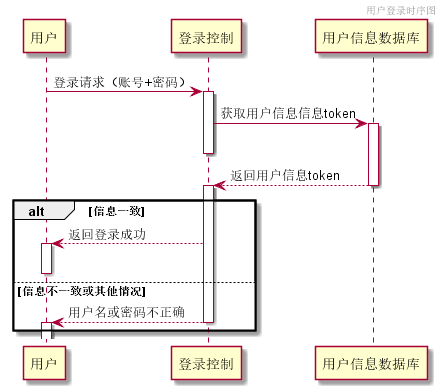
\includegraphics[width=0.8\textwidth]{用户登录时序图.pdf}
    \caption{用户登录时序图}
    \label{fig:用户登录时序图}
\end{figure}

用户注册时序图如\figref{fig:用户注册时序图}。

\begin{figure}[]
    \centering
    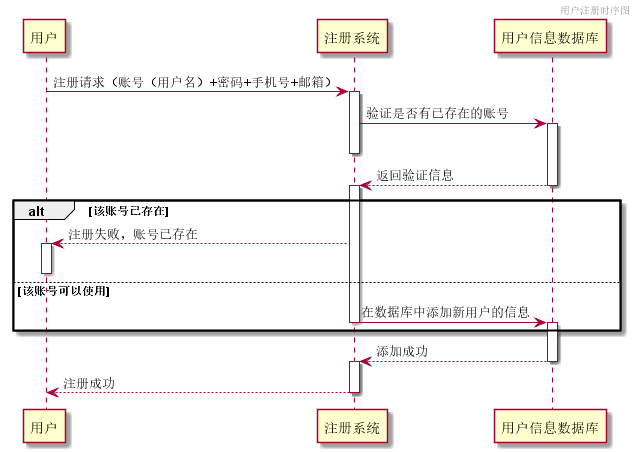
\includegraphics[width=0.8\textwidth]{用户注册时序图.pdf}
    \caption{用户注册时序图}
    \label{fig:用户注册时序图}
\end{figure}

房客订房时序图如\figref{fig:房客订房时序图}。


\begin{figure}[]
    \centering
    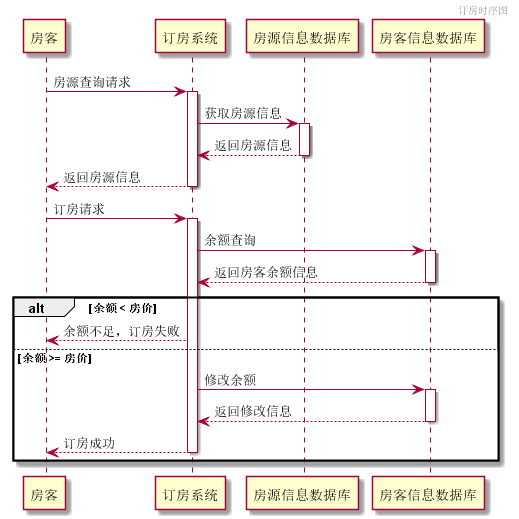
\includegraphics[width=0.8\textwidth]{房客订房时序图.pdf}
    \caption{房客订房时序图}
    \label{fig:房客订房时序图}
\end{figure}

房东上架房源时序图如\figref{fig:房东上架房源时序图}。

\begin{figure}[]
    \centering
    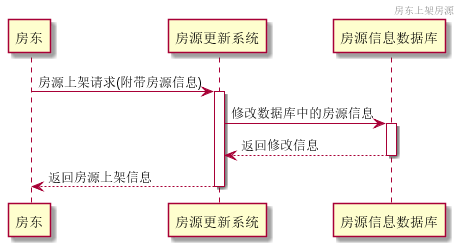
\includegraphics[width=0.8\textwidth]{房东上架房源时序图.pdf}
    \caption{房东上架房源时序图}
    \label{fig:房东上架房源时序图}
\end{figure}


房东下架房源时序图如\figref{fig:房东下架房源时序图}。

\begin{figure}[]
    \centering
    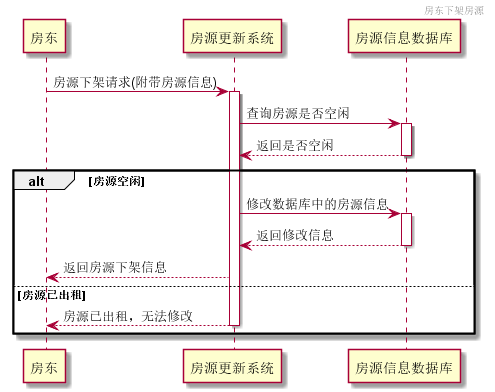
\includegraphics[width=0.8\textwidth]{房东下架房源时序图.pdf}
    \caption{房东下架房源时序图}
    \label{fig:房东下架房源时序图}
\end{figure}


房东更新房源时序图如\figref{fig:房东更新房源时序图}。

\begin{figure}[]
    \centering
    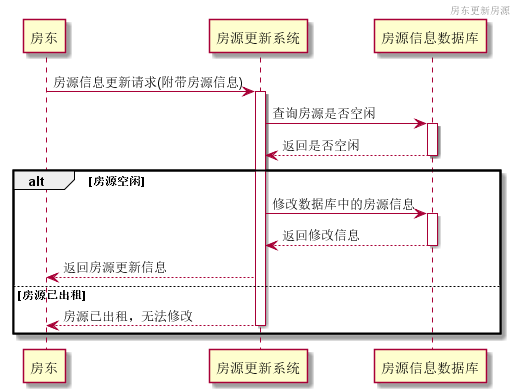
\includegraphics[width=0.8\textwidth]{房东更新房源时序图.pdf}
    \caption{房东更新房源时序图}
    \label{fig:房东更新房源时序图}
\end{figure}


\section{活动图}

动态图(activity diagram,活动图)是阐明了业务用例实现的工作流程。业务工作流程说明了业务为向所服务的业务主角提供其所需的价值而必须完成的工作。业务用例由一系列活动组成,它们共同为业务主角生成某些工件。工作流程通常包括一个基本工作流程和一个或多个备选工作流程。工作流程的结构使用活动图来进行说明。

工作流程活动图用于研究实现业务目标时所要执行的各项任务或活动的顺序安排。活动既可以是手动执行的任务,也可以是自动执行的任务。它可完成一个工作单元。活动图是状态图的一种特殊形式。其中所有或多数状态都是活动状态,而且所有或多数转移都在源状态中的活动完成时立即触发。

\subsection{房客登录活动图设计}

房客登录民宿预定系统时会进行以下操作:用户点击登录按钮,如果没有账号,则进行注册,输入新用户名,系统验证注册信息,数据库查询用户名是否已被注册,若已被注册则返回让用户重新输入新用户名,否则让用户输入密码,再次输入密码,输入邮箱号,系统向邮箱号发送验证码,用户输入验证码,提交注册信息,系统接收并传送注册信息,数据库将新用户信息添加入库;若已有帐号,则用户输入用户名,输入密码,系统验证登录信息,数据库比对用户名密码是否正确,若错误,则系统显示登陆失败,用户重新登陆,反之则显示登录成功,并显示主界面,以供用户继续操作。具体如\figref{fig:房客登录活动图}所示。

\begin{figure}[]
    \centering
    \includegraphics[width=0.8\textwidth]{房客登录活动图.pdf}
    \caption{房客登录活动图}
    \label{fig:房客登录活动图}
\end{figure}

\subsection{房东登录活动图设计}

房东登录民宿预定系统时会进行以下操作:用户点击登录按钮,若已有账号,则输入用户名,输入密码;否则进行注册,用户输入新用户名,系统验证注册信息,数据库查询用户名是否已被注册,若已被注册,则返回用户重新输入新用户名,否则,用户继续输入密码,再次输入以确认密码,输入邮箱号,系统向该邮箱号发送验证码,用户输入验证码,提交房东注册信息,系统进行房东信息审核,若审核未通过,则显示注册失败,反之则系统传送注册信息,数据库接受用户注册信息并添加入库,返回用户登录。具体如\figref{fig:房东登录活动图}所示。

\begin{figure}[]
    \centering
    \includegraphics[width=0.8\textwidth]{房东登录活动图.pdf}
    \caption{房东登录活动图}
    \label{fig:房东登录活动图}
\end{figure}

\subsection{房客订房活动图设计}

房客订房时会进行一下操作:用户进入搜索界面,输入关健词,点击搜索按钮,系统的搜索引擎获取关键词进入数据库,数据库进行数据检索,信息筛选,并返回给系统获得的信息,系统向用户显示搜索结果,用户挑选感兴趣的民宿,并点击查看,系统获取用户查看需求,数据库查询相应民宿,获取民宿的具体信息,系统向房客显示该民宿的具体信息,用户决定是否订购房屋,若是,则填写订购信息,系统核实订单,数据库修改该民宿信息,系统提示用户订房成功。具体如\figref{fig:房客订房活动图}所示。

\begin{figure}[]
    \centering
    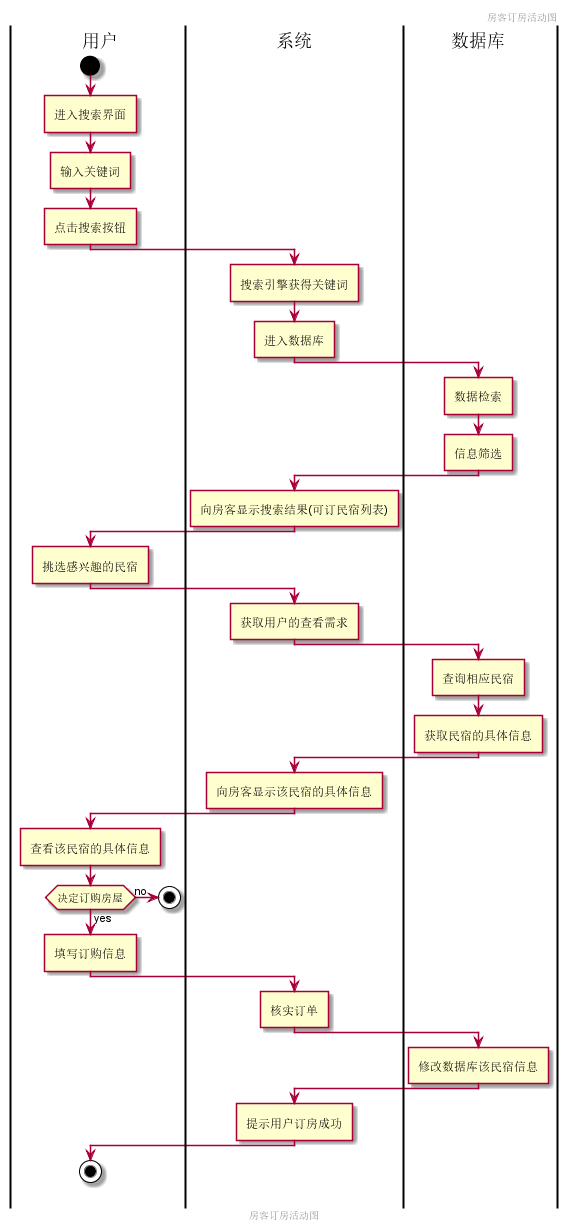
\includegraphics[width=0.8\textwidth]{房客订房活动图.pdf}
    \caption{房客订房活动图}
    \label{fig:房客订房活动图}
\end{figure}

\subsection{房东上架房源活动图设计}

房东提交房源信息的活动描述如下:用户进入房源信息提交界面,填写房源信息表格,点击提交按钮,系统审核用户提交的房源信息是否合格,若不合格,则向用户显示房源信息不合格,用户房源信息提交失败,若房源信息合格,则格式化房源信息,将房源信息添加入相应数据库,系统显示房源信息上传成功,并向用户显示房源信息提交成功。具体如\figref{fig:房东上架房源活动图}所示。

\begin{figure}[]
    \centering
    \includegraphics[width=0.8\textwidth]{房东上架房源活动图.pdf}
    \caption{房东上架房源活动图}
    \label{fig:房东上架房源活动图}
\end{figure}

\subsection{房源管理活动图设计}

民宿管理的活动描述如下:用户进入房源信息管理界面,选择需要操作的房源,系统判断该房源信息是否可以修改,若不可以修改,则显示房源信息修改失败,反之则显示房源可以修改,则用户进行房源信息的更新(修改价格、更新信息、下架房源等操作),系统获取房东修改指令,数据库检索相应房源,根据用户指令进行修改,若修改成功,返回给系统提示房东修改成功,否则显示房东修改失败,系统将修改结果返回给用户。具体如\figref{fig:房源管理活动图}。

\begin{figure}[]
    \centering
    \includegraphics[width=0.8\textwidth]{房源管理活动图.pdf}
    \caption{房源管理活动图}
    \label{fig:房源管理活动图}
\end{figure}

\section{课程设计心得及分工}

本次课程设计我们使用了\href{https://plantuml.com/zh/}{\textbf{plantuml}}这个工具来绘制uml图形,使用plantuml使我们可以将文本文件编译成精美的uml图片,同时plantuml支持非常多种类的图形绘制极大的加快了建模的过程。我们小组使用GitHub在疫情期间远程协作完成此次课程设计,所有的uml图片源码和需求分析文档都在\href{https://github.com/clysto/software-engineering}{\textbf{https://github.com/clysto/software-engineering}}这个项目中。

\subsection{心得}

在本次软件工程课程设计的过程中,我们将所学的理论知识与实际应用联系了起来,加深了对软件工程流程以及思想的理解。这次课设加深了我们对时序图、类图、用例图、活动图的认识以及它们各自的特点和使用方法,也提高了我们对软件开发的设计能力,以及绘制UML图的技能。小组合作模式,团队明确的分工和有效合作使任务清晰明了。我组首次尝试了在GitHub上构建项目流程,在很大的程度上提高了工作效率。


\subsection{分工}

\noindent
\begin{tabular}{@{}llp{10cm}}
    姓名 & 学号 & 分工\\ 
    王宇航 & 9173011818 &  部分用例图的补充、类图的设计与绘制、时序图的设计与绘制、对应部分报告的编写\\ 
    毛亚琛 & 9173011613 &  用例图的设计与绘制、GitHub项目的构建、对应部分报告的编写、总体报告排版与整理\\ 
    朱志畅 & 30217331   &  活动图的设计与绘制、项目背景的提出、需求分析、功能分析、性能分析、对应部分报告的编写\\ 
\end{tabular}


\end{document}
